\chapter{Modellierung}
\label{sec:modellierung}
Im mathematischen Modell werden die Anforderungen aus der Trainingswissenschaft in das Format der Constraint Programmierung übersetzt. Die Modellierung optimiert jeden Monat gesondert nach Anteilen der Belastungbereiche und berechnet deshalb die Trainingseinheiten für einen Zeitraum von 28 Tagen. Zur Auswahl stehen dabei Einheiten der verschiedenen Trainingsmethoden, um wochenweise die Trainingsumfänge zu füllen. Dauer, Methode und Belastungsbereiche charakterisieren eine Einheit. Später werden die Mesozyklen zu einem Makrozyklus verbunden, der den gesamten Trainingsplan widerspiegelt.
\begin{figure}[h]
    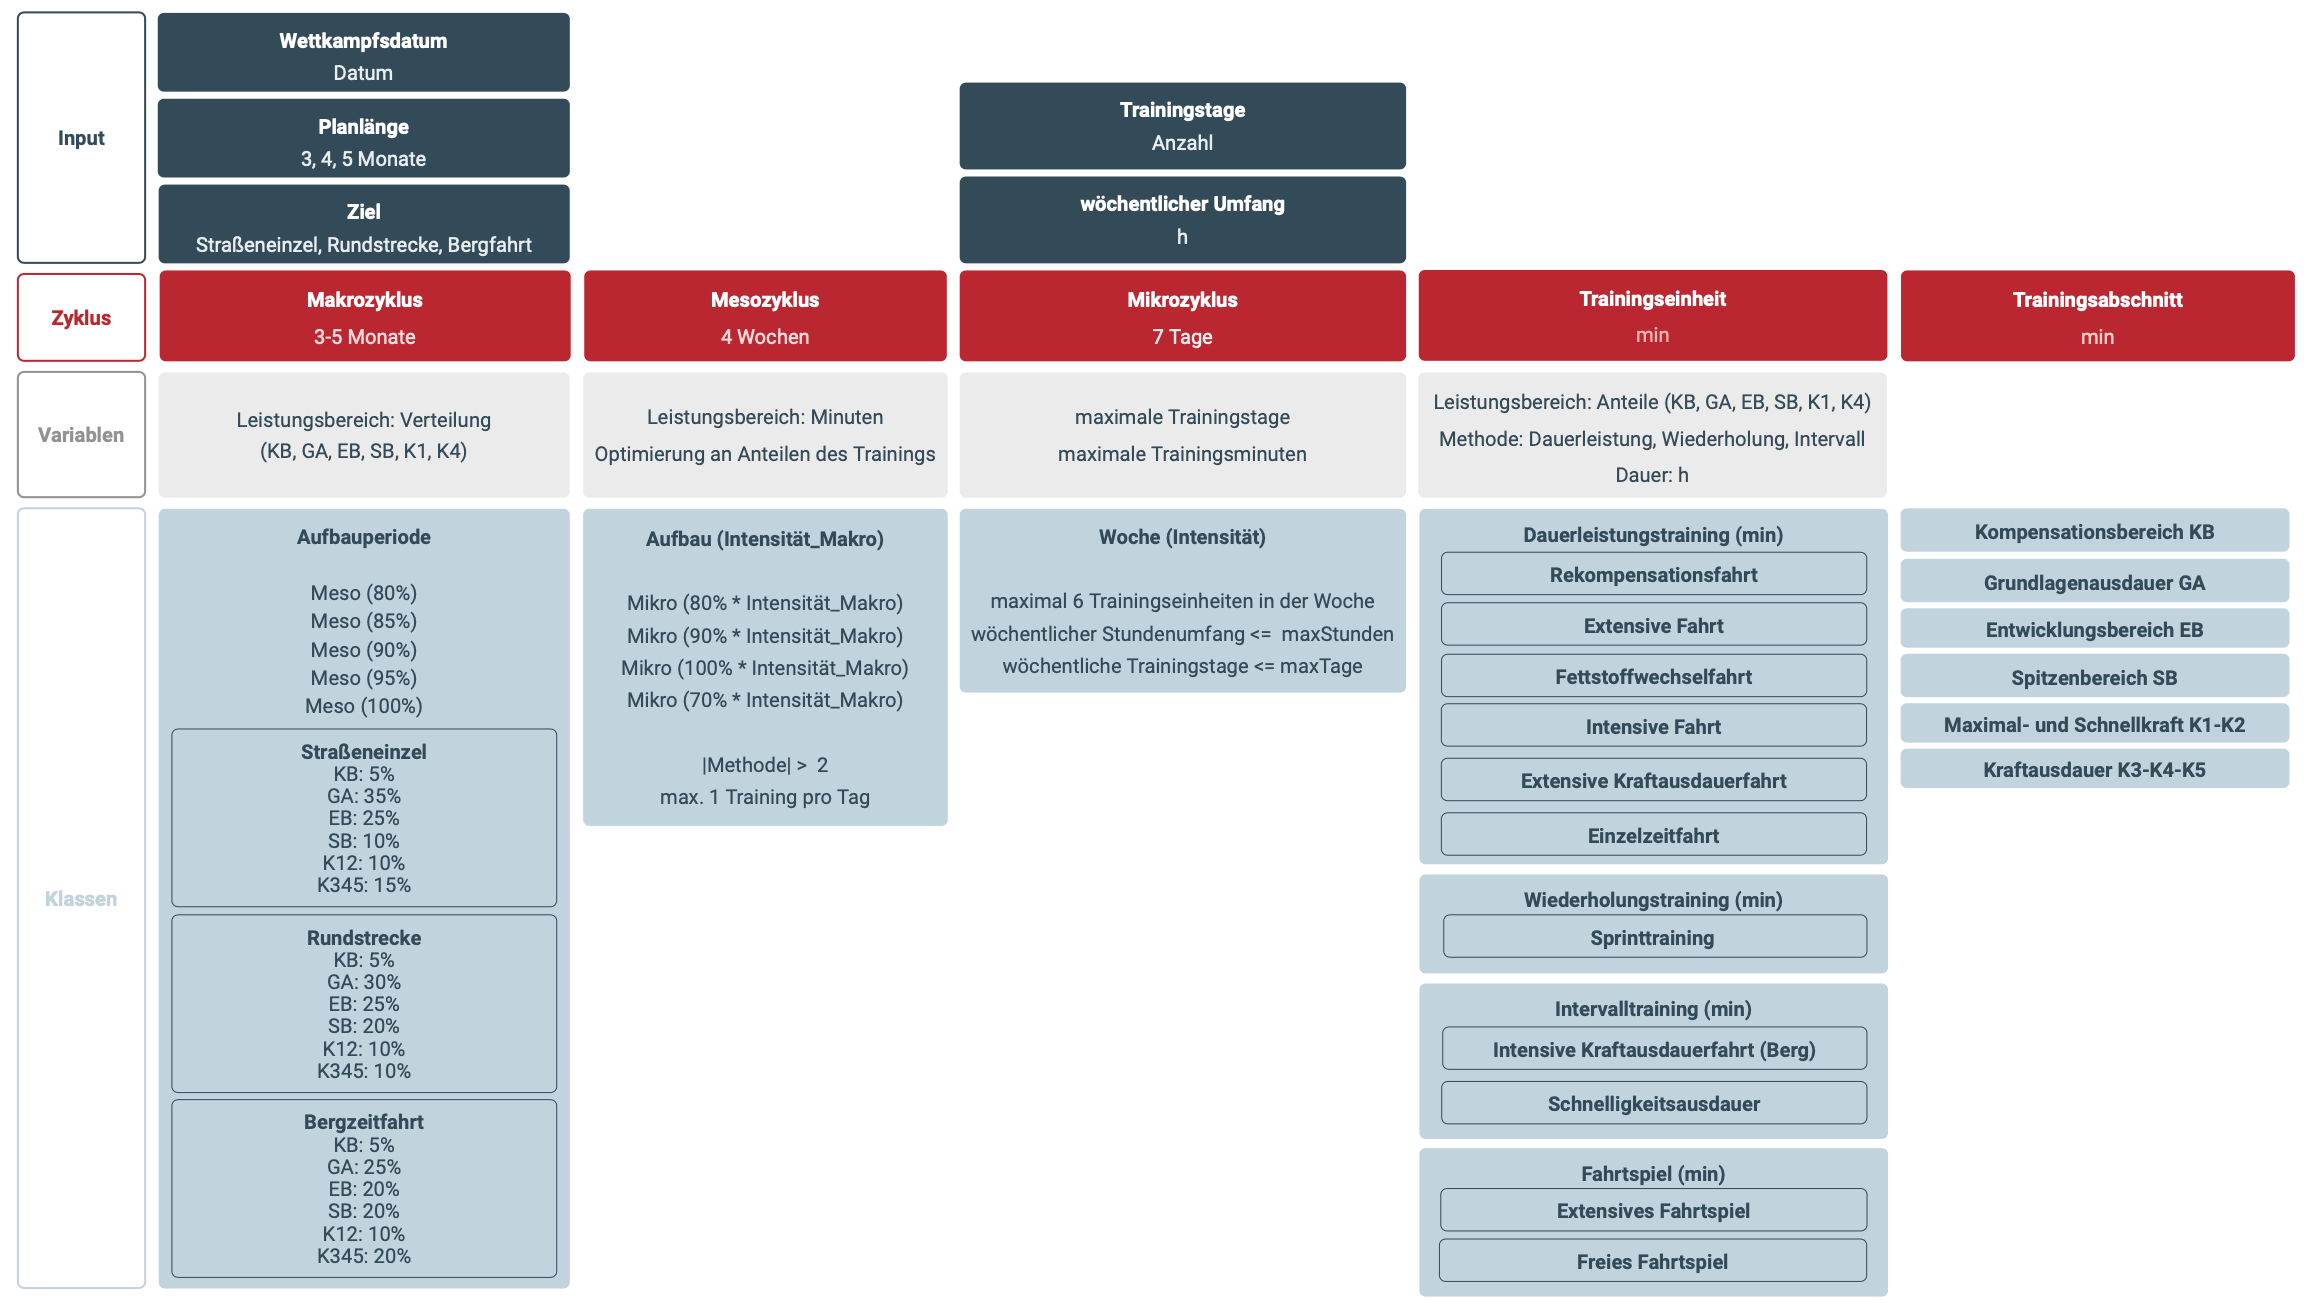
\includegraphics[width=\textwidth,height=\textheight, keepaspectratio]{gfx/modellierung.png}
    \caption{Schema der Modellierung mit hierarchischer Struktur (\hyperref[anhang:modellierung:gross]{siehe \ref{anhang:modellierung:gross}})}
    \label{abbildung:modellierung:schema}
\end{figure}
\section{Designprozess}
Im ersten Ansatz der Modellierung eines Trainingsplans wurde kein kombinatorischer Grundgedanke verfolgt. Statt einer Menge an validen Trainingseinheiten, definierte das System die Charakteristika einer Trainingsmethode. Die Schwierigkeit ist jedoch, die vielen Einzelfälle und Ausnahmen präzise genug abzudecken, ohne ein sehr unübersichtliches Constraint-System zu erhalten. Besonders im Hinblick auf die Erweiterung und Skalierbarkeit scheiterte dieser Versuch. Stattdessen wird das Problem als kombinatorische Optimierung betrachtet, das die einzelnen Trainingseinheiten mit dynamischer Verteilung der Belastungsbereiche definiert und nach Prinzipien der Sportwissenschaften kombiniert. Es gelten wochen- und monatsweise Kriterien, die erfüllt sein müssen. Ein weiterer Vorteil ist die einfache Erweiterung um weitere Arten von validen Trainingseinheiten, siehe \ref{anhang:einheiten}. Die Benennung in der Liste der annehmbaren Verteilungen konkretisiert auch die Darstellung in der Ausgabe. \newline
Des Weiteren wurde von einer Modellierung auf Basis von Kraft, Ausdauer und Schnelligkeitsanteilen abgesehen. In diesem Fall wären Schätzungen an zwei Stellen vonnöten. Erst müssen für die Trainingseinheiten die drei Bereiche festgelegt werden und dann, wie auch in der aktuellen Modellierung, die Gewichtung in Abhängigkeit der Wettkampfdisziplin. Mit Definition einer Trainingseinheit über die Belastungsbereiche selbst kann die Schätzung an einer Stelle gebündelt werden. Die Wettkampfarten dienen als Vorlage für die Verteilung, sind von der Modellierung aber unabhängig festgelegt. \newline
Die Optimierung auf Ebene der Mesozyklen erlaubt der Verteilung und Variation genug Spielraum. Die Gefahr einer wochenweisen Optimierung ist, dass es eine Lösungsinstanz gibt, die für alle Wochen in sehr ähnlicher Form verwendet wird. Die Variation lässt sich damit nicht genügend steuern. Anhand der monatlichen Kapselung wirkt man der Monotonie entgegen und die Erstellung eines Trainingsplans kann dennoch in ausreichend kleine Teilprobleme zerlegt werden.

\section{Modell}
\label{sec:modellierung:model}
Die verschiedenen Ebenen des Modells gleichen denen der Zyklisierung. Die Struktur ist in \hyperref[abbildung:modellierung:schema]{Abbildung \ref{abbildung:modellierung:schema}} visualisiert. Ein Trainingsplan betrifft in der Modellierung die Aufbauperiode. Hier gibt es je nach Wettkampfdisziplin drei verschiedene Ausprägungen. Bewertet wird die Relevanz der Belastungsbereiche durch deren Auswahl. Eingebettet in einen Makrozyklus sind mehrere Mesozyklen. Abhängig von der Planlänge werden hier die Intensitäten und Umfänge angepasst. Ein Mikrozyklus teilt die vier Wochen ein. Hier kommen Beschränkungen der Umfänge zum Tragen. Die Trainingseinheiten einer Woche sind gruppiert nach ihren Methoden. Identisch zu \ref{anhang:einheiten} wurden die einzelnen Trainingsabschnitte dynamisch definiert.
\begin{enumerate}[parsep=2pt, topsep=0pt]
    \item Makrozyklus aus Wettkampfdisziplin bestimmen 
    \item Anzahl an Mesozyklen je nach Dauer einbetten
    \item Vorgaben der Umfänge berechnen und an Mesozyklen weitergeben
    \item Mesozyklen modellieren je 28 Tage aus den verfügbaren Trainingseinheiten
    \item Optimierung anhand der Distanz zu den Belastungsbereichen
    \item Erstellte Trainingseinheiten aus den Mesozyklen zusammensetzen
\end{enumerate}

\subsection{Konstanten}
In der Modellierung werden Konstanten gesondert betrachtet. Diese Größen sind in jeder Lösungsinstanz relevant, aber vor der Modellierung fest bestimmt. 

In $maxminutes_i$ ist die Beschränkung der Trainingsminuten der i-ten Woche festgesetzt. In diesem Modell wird eine Trainingswoche auf maximal zwölf Stunden begrenzt. Bereits vor dem Lösen des Modells ist die 3:1 Periodisierung in diesen Variablen festgehalten. Die vier Wochen des Mesozyklus werden progressiv gestaltet und die Umfänge betragen 80 \%, 90 \%, 100 \% und 70 \% des Umfangs ihres Makrozyklus. Mit dieser Methode ist auch sichergestellt, dass zum Ende des Plans -- und damit in der Woche vor dem Wettkampf -- eine Regenerationswoche eingeplant wird.
\begin{equation}
     maxminutes_w \in [0, 300] , \forall w \in \{0, 1, 2, 3\}
\end{equation}
Analog dazu gibt es auch eine Begrenzung der Trainingstage einer Woche. Die Anforderung an mindestens einen Regenerationstag ist hier umgesetzt, da die Trainingstage maximal sechs Tage betragen können. Dieses Limit gilt für jede der vier Wochen.
\begin{equation}
\label{equation:maxDays}
     maxdays \in [2, 6]
\end{equation}
Maßgeblich für die Optimierungsvariable sind die festgesetzten Ziele je Belastungsbereich $R = \{kb, ga, eb, sb, k1, k4\}$. Sie werden aus den Anforderungen eines Wettkampfs und den zur Verfügung stehenden Trainingsminuten berechnet. Wichtig ist hier, die zyklischen Wochenumfänge prozentual einzubeziehen, damit die vorgegebenen Minuten in den Bereichen auch mit den wöchentlichen Begrenzungen erreichbar sind.\newline
Die Periodisierung des Trainingsplans kann damit ebenfalls gesteuert werden. Je näher die Monate am Datum des Wettkampfs liegen, desto höher wird die wettkampfspezifische Belastung gewichtet. Auch dieses Prinzip wird schon vor der Modellierung durch den Makrozyklus umgesetzt. 
\begin{equation}
    target_{r} \in [0, 300*4*6] , \forall r \in R
\end{equation}
\subsection{Variablen}
Unter den Variablen der Modellierung werden die veränderlichen Größen verstanden. Die endlichen Wertebereiche sind möglichst präzise zu wählen, um den Suchraum zu verkleinern. Eine Lösungsinstanz definiert die Belegung der Variablen mit konkreten Werten für jeden Tag des Mesozyklus:  $\forall i \in [0, 27]$.\par
\textbf{Name der Einheit} \\[0.2em]
Variable für die Identifikation der Trainingseinheit am Tag $i$. Die Liste der Trainingseinheiten wird durch eine 1:1-Korrespondenz (siehe \ref{anhang:trainingsarten}) abgebildet.
\begin{equation}
    name_i = [\![0, 11]\!]
\end{equation}
\textbf{Dauer einer Einheit} \\[0.2em]
Variable für die Dauer der Trainingseinheit an Tag $i$ in Minuten. Es wird für einen Tag eine maximale Trainingszeit von fünf Stunden angesetzt.
\begin{equation} 
    duration_i = [\![0, 300]\!] \end{equation} 
\textbf{Trainingsmethode einer Einheit} \\[0.2em]
Variable für die Trainingsmethode der Trainingseinheit an Tag $i$. Für Tage ohne Trainingseinheit wird die Methode \textit{PAUSE} eingeführt. Auch wenn durch den Namen der Trainingseinheit ein direkter Zusammenhang mit der Methode besteht, wird diese explizit definiert, um die Variation der Trainingsmethoden zu gewährleisten.
\begin{equation}
    method_i \in M
\end{equation} 
\textbf{Belastungsbereiche einer Einheit} \\[0.2em]
Variable für die Minuten je Belastungsbereich $r \in R$ an Tag $i$. Sie wird für alle Elemente aus $\{kb, ga, eb, sb, k1, k4\}$ definiert. Die maximale Trainingszeit gilt hier gleichermaßen, da ein Training bei der Dauerleistungsmethode in nur einem Bereich absolviert werden kann. \newline
\begin{equation} 
    r_i = [\![0, 300]\!]
\end{equation} 
\subsection{Constraints}
\subsubsection{Constraints für Trainingstage}
Für die Definition der Constraints werden Tage durch $i \in [0, 27]$ identifiziert. \par
\textbf{Diskretisierung der Trainingseinheiten} \\[0.2em]
Die Trainingseinheiten werden bei ihrer Länge auf viertelstündliche Abschnitte diskretisiert. Das verkleinert den Wertebereich der Variablen um 93,3 \%, ohne die mögliche maximale Länge der Einheiten zu kürzen. Die Trainingseinheiten sind im Hinblick auf den Anwendungsfall so auch praxistauglich.
\begin{equation}
    {duration}_i \mod 15 = 0
\end{equation} 
\textbf{Diskretisierung der Trainingsbereiche} \\[0.2em]
Gleiches gilt für die Trainingsbereiche $R = \{kb_i, ga_i, eb_i, sb_i, k1_i, k4_i\}$ einer Einheit. In 15-minütigen Abschnitten festgesetzt, bieten sie genug Genauigkeit für den Benutzer, ohne einen sehr großen Suchraum zu erzwingen. Die Definition der Abschnitte in minütlicher Genauigkeit bietet keinen erheblichen Mehrwert. Der kleinere Wertebereich kommt der Implementierung in \hyperref[sec:implementierung]{Kapitel \ref{sec:implementierung}} zugute, ohne die Erstellung auf sehr kurze Traininingseinheiten zu limitieren.
\begin{equation}
    r_i \mod 15 = 0, \forall r \in R
\end{equation}
\textbf{Konsistenz von Dauer der Einheiten und Trainingsabschnitten} \\[0.2em]
Für jeden Trainingstag $i$ mit Trainingsabschnitten in den Bereichen $r \in R$ gilt, dass deren Summe auch der Länge des Trainings entspricht.
\begin{equation}
    \sum_{r\in R} r_i = duration_i
\end{equation}
\textbf{Variation der Trainingsmethoden} \\[0.2em]
Um die Variation der Trainingsmethoden $M = \{PAUSE, DL, FS, IV, WH\}$ zu garantieren, wird verlangt, dass jede Trainingsmethode mindestens zwei Mal verwendet wird. Durch die vier Trainingsmethoden wird eine Mindestanzahl von zwei Trainingstagen pro Woche benötigt, um ein lösbares System zu erhalten. Das ist durch die Wertebereiche von $maxdays$ in \ref{equation:maxDays} sichergestellt.
\begin{equation} 
    |\{method_i = m\}| \geq 2, \forall m \in M
\end{equation} 
\textbf{Definition von Pause} \\[0.2em]
Ist an einem Tag die Trainingsdauer auf Null gesetzt, entspricht das einer Pause im Trainingsplan. Die Pause als Trainingsmethode umzusetzen, erlaubt es, immer 28 Tage zu modellieren.
\begin{equation}
    method_i = \text{PAUSE} \Leftrightarrow duration_i = 0
\end{equation}
\textbf{Menge der validen Trainingseinheiten} \\[0.2em]
Wie bereits in Abschnitt \ref{grundlagen:methoden} definiert, werden die möglichen Trainingseinheiten einer Methode als Menge vorgegeben. Minimum und Maximum der Belastungsbereiche legen die erlaubte Zeitspanne fest. Exemplarisch am Fahrtspiel gelten damit folgende Bedingungen für die geordnete Menge $ranges_i = (kb_i, ga_i, eb_i, sb_i, k1_i, k4_i)$. Die vollständige Modellierung für alle Trainingsmethoden erfolgt analog nach den definierten Trainingseinheiten. Sie befindet sich im Anhang \ref{anhang:modell}.
\begin{equation}
    (method_i = \text{Fahrtspiel})\Rightarrow t_i = \begin{array}{c}
            (0, [\![60, 240]\!], [\![60, 240]\!], 0, 0, 0) \\ 
        \vee (0, [\![60,180]\!], [\![60, 180]\!], [\![60, 180]\!], 0, 0)
    \end{array}
\end{equation}
\subsubsection{Constraints für Trainingswochen}
Folgende Constraints gelten für alle Wochen $w \in \{0, 1, 2, 3\}$ des Mesozyklus.\par
\textbf{Limitierung des wöchentlichen Stundenumfangs} \\[0.2em]
Die Summe der Trainingsstunden muss unter dem vorgegebenen wöchentlichen Umfang liegen. Dieser beinhaltet bereits die Periodisierung des Plans.
\begin{equation}
    \sum_{j=7*w}^{7*w+6} duration_j \leq maxminutes_w
\end{equation}
\textbf{Limitierung der wöchentlichen Trainingstage} \\[0.2em]
Ähnlich verhält es sich bei den limitierten Trainingstagen in einer Woche. Hier ist der Schwellenwert für alle Wochen identisch und durch die Konstante $maxdays$ vorgegeben. Die Modellierung erlaubt es, den Wert um einen Tag zu unterschreiten, um die Verteilung der Einheiten flexibel zu halten. 
\begin{equation}
    \sum_{j=7*w}^{7*w+6}  (duration_j > 0) \leq maxdays
\end{equation}
\subsection{Optimierung}
Die Modellierung berechnet die Summe der Trainingsminuten in den verschiedenen Belastungsbereichen. Die Distanz dieser zu der kalkulierten Vorgabe wird summiert und als Abweichung des Modells festgelegt. Mithilfe dieser Größe wird die Güte einer Lösungsinstanz quantifiziert. Das Modell strebt bei der Lösung die Minimierung dieses Wertes an.
\begin{equation}
    \text{minimize} \sum_{r\in R} |target_r - \sum_{i=0}^{28}r_i|
\end{equation} 
